
\documentclass[	paper=a4, twoside = true, fontsize = 12,  % font size for \normalsize set to 12
				% parskip = half,  % paragraphs are separated by 0.5\baselineskip
				% BCOR = 0cm,  % sets bonding correction (Bindekorrektur) to 0 cm
				toc = bibliography,  % add bibliography to table of contens
				numbers = noendperiod,  % no dot at the end of chapter and section labels
				english,  % set language to english
			]{scrbook}  % document class

% ################################################
% Definitions
% ################################################
\def\DRAFT{} % comment out for the finished document!
\def\myTypeOfDocument{Dissertation}
\def\myAuthor{Florian Kleiner}  % authors name
\def\myUniversity{Bauhaus-Universität Weimar}
\def\myFirstReviewer{Professor Dr.-Ing. Horst-Michael Ludwig}  % name of first reviewer
\def\mySecondReviewer{Unknown}  % name of second reviewer
\def\myThirdReviewer{Unknown}   % name of second reviewer
\def\myExamDate{xx.xx.2025}
\def\myTitle{2D and 3D characterization of clinker phases and hydrated cementitious binders by a variety of modern imaging techniques}
%\def\mySubtitle{(Arbeitstitel)}

% ########################
% Load necessary packages
% ########################

\RequirePackage{babel}[2020/10/27]  % set language via option in document class

\usepackage[%
			%headsepline,  % plotted line under each headline
			%plainheadsepline,  % plotted line over each headline even on plain pages (chapter beginning)
			%footsepline,  % plotted line over each footline
			plainfootsepline  % plotted line over each footline even on plain pages
			]{scrlayer-scrpage}  % package for manipulating headlines
%ihead{\Ifstr{\leftmark}{\rightmark}{}{\rightmark}}
%\ohead{\pagemark}
%\ofoot*{\pagemark}

\usepackage[inner = 3cm,
			outer = 2.5cm,
			top = 3.25cm,
			bottom = 3cm
			]{geometry}  % manipulate page margins

\usepackage{setspace}  % change linespacing

\usepackage[T1]{fontenc}  % changed font encoding to west-european letters
\usepackage{textalpha}  % use greek letters in text directly like α -> package textgreek
\usepackage{lmodern}  % modification of fonts to make them 'clearer'
\usepackage{textcomp}  % eg. modified € und § symbols
\usepackage{csquotes}  % provides advanced facilities for inline and display quotations

%\usepackage[scaled]{uarial}  % Use Arial-clone font as sffamily-font

\usepackage{xcolor}  % makes latex more colorful

\usepackage{microtype}  % Better results in line breaks and overfull boxes
%error

\usepackage[labelsep=quad,  % Add a \quad after caption label
			format=hang,  % Captionlabels with multiple lines are hanging
			font={footnotesize, sf},  % changing font for caption label and
			%text
			labelfont=bf  % changing font only for caption text
			]{caption}  % additional options for captions and required for subcaption package

\usepackage{subcaption}  % includes subfigure environment

\usepackage{amssymb}
\usepackage{amsmath}  % highly improves math mode
\usepackage{booktabs}  % beautify tables
\usepackage{longtable}  % environment to create tables of a length of multiple pages
\usepackage{tabularx}  % create tabulars with a fixed width (one flexible col)
\usepackage{pdfpages}  % include multiple pages of pdf documents
\usepackage{lscape}  % introduced the landscape environment to turn tables landscape

\usepackage{datetime}
\newdateformat{myDateFormat}{\THEDAY. \monthname[\THEMONTH] \THEYEAR}
\def\myCompileDate{\myDateFormat\today}

\ifdefined\DRAFT
	\usepackage[firstpageonly=true,
				scale=5,
				fontsize=12pt, % DO NOT REMOVE, else the package will generate an error
				]{draftwatermark}
\fi

\usepackage{todonotes}  % creates to-do items and figures

%%%%%% Hyperref Settings
\ifdefined\DRAFT
	\def\myTypeOfDocumentPDF{\myTypeOfDocument (Draftversion)}
\else
	\def\myTypeOfDocumentPDF{\myTypeOfDocument}
\fi

\usepackage[hidelinks,  % hide links in pdf document
			pdftitle    = {\myTitle},
			pdfsubject  = {\myTypeOfDocumentPDF},
			pdfauthor   = {\myAuthor},
			%pdfproducer = {\myUniversity},
			]{hyperref}

\usepackage{graphicx}  % include graphics

\usepackage[style = numeric-comp,
			backend=bibtex,
			maxbibnames = 99, % arbitrary high value to ensure that all authors are listet in the bibliography
			maxcitenames = 2, % truncate nameslist for citations
			giveninits = true, % abbrevation for first name
			date = year, % controls the basic format of printed date specifications
			uniquelist = false, % This feature allows ambiguous labelname list --> unique dateformat (e.g. 2020a, 2020b)
			]{biblatex}  % use biblatex for bibliography

\usepackage[range-units=single  % on default show only a single unit when using /SIrange{}
			]{siunitx}  % helpfull to show value-unit-pairs in text

\usepackage{enumitem}  % improves enumerate and itemize environment

\usepackage{ziffer}  % conversion of punctuation in maths mode (switches . and ,)
\usepackage{lineno}  % create line numbering for review process
\usepackage{blindtext}  % creates blindtexts
\usepackage{nicefrac}
\usepackage{textgreek}

\usepackage[printonlyused]{acronym} % nohyperlinks
\usepackage{etoolbox}
\makeatletter
\expandafter\patchcmd\csname AC@\AC@prefix{}@acro\endcsname{{#3}}{{\MakeUppercase #3}}{}{}
\expandafter\patchcmd\csname AC@\AC@prefix{}@acro\endcsname{{#3}}{{\MakeUppercase #3}}{}{}
\makeatother

% ########################
% Define page design
% ########################

% Define formatting of headlines
\setkomafont{chapter}{\Large\sffamily}
\setkomafont{section}{\large\sffamily}
\setkomafont{subsection}{\normalsize\sffamily}
\setkomafont{subsubsection}{\normalsize\sffamily}
\setkomafont{pageheadfoot}{\footnotesize}
\setkomafont{pagefoot}{\usekomafont{pageheadfoot}}
\setkomafont{pagenumber}{\usekomafont{pageheadfoot}}
\addtokomafont{disposition}{\rmfamily}
\setcounter{secnumdepth}{\subsubsectionnumdepth}  % activate numbering of subsubsection

% Define header
\clearpairofpagestyles  % clear existing header and footer
% without *: only on regular pages
% with *: also on plain pages (like chapter beginning)
\ohead{\sffamily\headmark}  % Inside show caption of chapter (left) / section (right); [\sffamily\leftmark] on plain pages allways chapter (leftmark)

% Define footer
%\ifoot*{\sffamily Dissertation \myAuthor}  % Show authors name
\ofoot*{\sffamily\pagemark}  % Show page number

% Set line spacing to 1.15
\setstretch{1.15}

% Set parskip to 0.25 instead of half or full
\setparsizes{0em}{0.25\baselineskip plus .25\baselineskip}{1em plus 1fil}

% Disable single lines at the start of a paragraph (orphans)
\clubpenalty = 10000
% Disable single lines at the end of a paragraph (widows)
\widowpenalty = 10000 \displaywidowpenalty = 10000

% Defaults for figure environments
\setkeys{Gin}{keepaspectratio=true}  % allways keep aspact ratio of figures

% Define enumerate end itemize environment defaults
\setlist{nosep, itemsep=0.3ex}  % set margin of enumerate and itemize environment
\setlist[itemize]{label=--}  % set itemize label to dash


% ########################
% Define predefined colors
% ########################
\definecolor{grey}{rgb}{0.8,0.8,0.8}  % Define grey


% ########################
% Table enhancements
% ########################

% Adding new columntypes with option of width specification and vertical centering
% Example: \begin{tabular}{L{4.0cm}C{3cm}}
\newcolumntype{L}[1]{>{\raggedright\arraybackslash}m{#1}} % flush left with  width specification
\newcolumntype{R}[1]{>{\raggedleft\arraybackslash}m{#1}} % flush right with  width specification
\newcolumntype{C}[1]{>{\centering\arraybackslash}m{#1}}  % centered with  width specification

% ################################################
% Language setup for siunitx
% ################################################
\addto\extrasngerman{\sisetup{locale = DE}}
\addto\extrasenglish{\sisetup{locale = US}}

% ################################################
% Additional user settings
% ################################################
\graphicspath{{figures/}}  % define graphics standard path
%\input{additionals/acronyms}  % import acronyms


\renewcommand*{\chapterformat}{%
\mbox{\chapappifchapterprefix{\nobreakspace}%
\scalebox{3}{\color{gray}\thechapter\autodot \color{black}$\vert$}\enskip}}
  % import packages and design definitions
\def\myCompileDate{\myDateFormat\today}

\addbibresource{Dissertation.bib}

\begin{document}

	\begin{titlepage}
	%\vspace*{1\baselineskip}
	\rmfamily{

		{\centering
			{\LARGE\textbf{\myTitle}\par}
			\centering
			%\vspace*{0.2\baselineskip}
			%{\large \textbf{\mySubtitle}}

			\vspace*{3\baselineskip}
			\Large\uppercase{Dissertation}\large

			\vspace*{1\baselineskip}
			zur Erlangung des akademischen Grades

			Doktor-Ingenieur (Dr.-Ing.)

			\vspace*{2\baselineskip}
			an der Fakultät für Bauingenieurwesen der

			\Large\textsc{\myUniversity}\large

			\vspace*{2\baselineskip}
			vorgelegt von

			Dipl.-Ing. \myAuthor

			\vspace*{1\baselineskip}

			geboren am 31.07.1987 in Leinefelde, Deutschland

		}


		\vspace*{3\baselineskip}
		\begin{tabbing}
			Stand des Dokumentes:	\=	Name \kill
			Gutachter:	\>	\myFirstReviewer \\
						\>	\mySecondReviewer \\
						\>	\myThirdReviewer
			\end{tabbing}

			\begin{tabbing}
			Stand des Dokumentes:	\=	Name \kill
			Tag der Disputation: \>	\myExamDate \\
			\ifdefined\DRAFT
				Stand des Dokumentes: \>	\myCompileDate
			\fi
		\end{tabbing}
	}
\end{titlepage}  % include correct title page

	\frontmatter  % start front matter section
		\pagenumbering{Roman}  % set page numbering to Roman

		\chapter*{Acknowledgements (Danksagung)}
\selectlanguage{german}
Die vorliegende Dissertation entstand während meiner Tätigkeit als wissenschaftlicher Mitarbeiter
am F. A. Finger-Institut für Baustoffkunde, Professur Werkstoffe des Bauens an der Bauhaus-Universität Weimar im Rahmen mehrerer von der DFG geförderter Projekte.

An dieser Stelle möchte ich mich bei allen bedanken, die zum Gelingen dieser Arbeit beigetragen haben. Mein herzlicher Dank gilt Christiane Rößler für die fachliche Unterstützung und Motivation und den angehörigen der Arbeitsgruppe Zementchemie und Rasterelektronenmikroskopie. Insbesondere Christian Matthes für die gemeinsamen Untersuchungen an den Rasterelektronenmikroskopien sowie Lydia Schmiedel und Nadine Brendel für die Politur zahlreicher Proben.

[...]

Abschließend möchte ich mich bei meinen Freunden und KollegInnen bedanken, die mich aif dem Weg meines Promotionsstudiums immer wieder zur Arbeit an diesem Dokument motivieren konnten.
		\tableofcontents  % print table of contents
		\chapter{List of Acronyms}

\begin{acronym}

\acro{CSH}[C-S-H]{calcium silicate hydrates}
\acro{CH}[CH]{portlandite}
\acro{C3S}[C$3$S]{tricalcium silicate}
\acro{C2S}[C$2$S]{dicalcium silicate}
\acro{SEM}[SEM]{scanning electron microscope}
\acro{FIB}[FIB]{focussed Ion Beam}
\acro{EDX}[EDX]{energy-dispersive X-ray spectroscopy}
\acro{EBSD}[EBSD]{electron backscatter diffraction}
\acro{BSE}[BSE]{backscattered electrons}
\acro{XRD}[XRD]{X-ray diffraction}

\end{acronym}

\chapter{List of Symbols}

\begin{longtable}[l]{p{1.5cm}p{1.5cm}p{0.7\linewidth}}
	$A_0$ & $[m^2]$ & Querschnittsfläche zu Beginn des Versuches \\
	$B$ & $[m]$ & Probenbreite\\
	$c$ & $[Pa]$ & Kohäsion (Mohr-Coulomb'sches Stoffgesetz) \\
	$\alpha$ & $[-]$ & Radius des Übergangsbereiches $F_s$ \\
	$\gamma$ & $[^\circ]$ & Wandneigungswinkel \\
	$\beta$ & $[^\circ]$ & Reibungswinkel (Cap-Plasticity Stoffgesetz) \\
\end{longtable}  % include list of symbols


	% Helpfull features for review process
	%\linenumbers  % add numbers to each line
	%\setstretch{2}  % set line spacing to factor 2
	\mainmatter  % start main matter (arabic page numbering)

		%Einleitung (SEM/Zement/Bildverarbeitung)
		%Methodik/Theorie (SEM/Kategorisierung von Zementen?)
		%Ergebnisse
		%- Unterkapitel 1,2,3,4...
		%Zusammenfassung

		\chapter{Introduction}

\section{Background and Motivation}

Portland cement is the most commonly used binder for the production of concrete.
After adding water to the cement, a reaction called `hydration' begins.
The cement reactivity is determined by its composition and particle size.
During hydration, the cement begins to dissolve and new crystals start to form (see Figure~\ref{fig:intro}).
This ultimately causes hardening of the cement paste.
Furthermore, this microstructure determines the properties of the resulting concrete.

In 1929 \textsc{Anderegg} and \textsc{Hubbell} introduced their paper as follows:
\begin{iquote}
	The lack of knowledge concerning the rate of hydration of cement clinker has hindered a more complete understanding of the complicated setting and hardening reactions that cements undergo. \cite{anderegg.1929}
\end{iquote}


\begin{figure*}[b!]
    \centering

	\ifdefined\PRINTABLE
		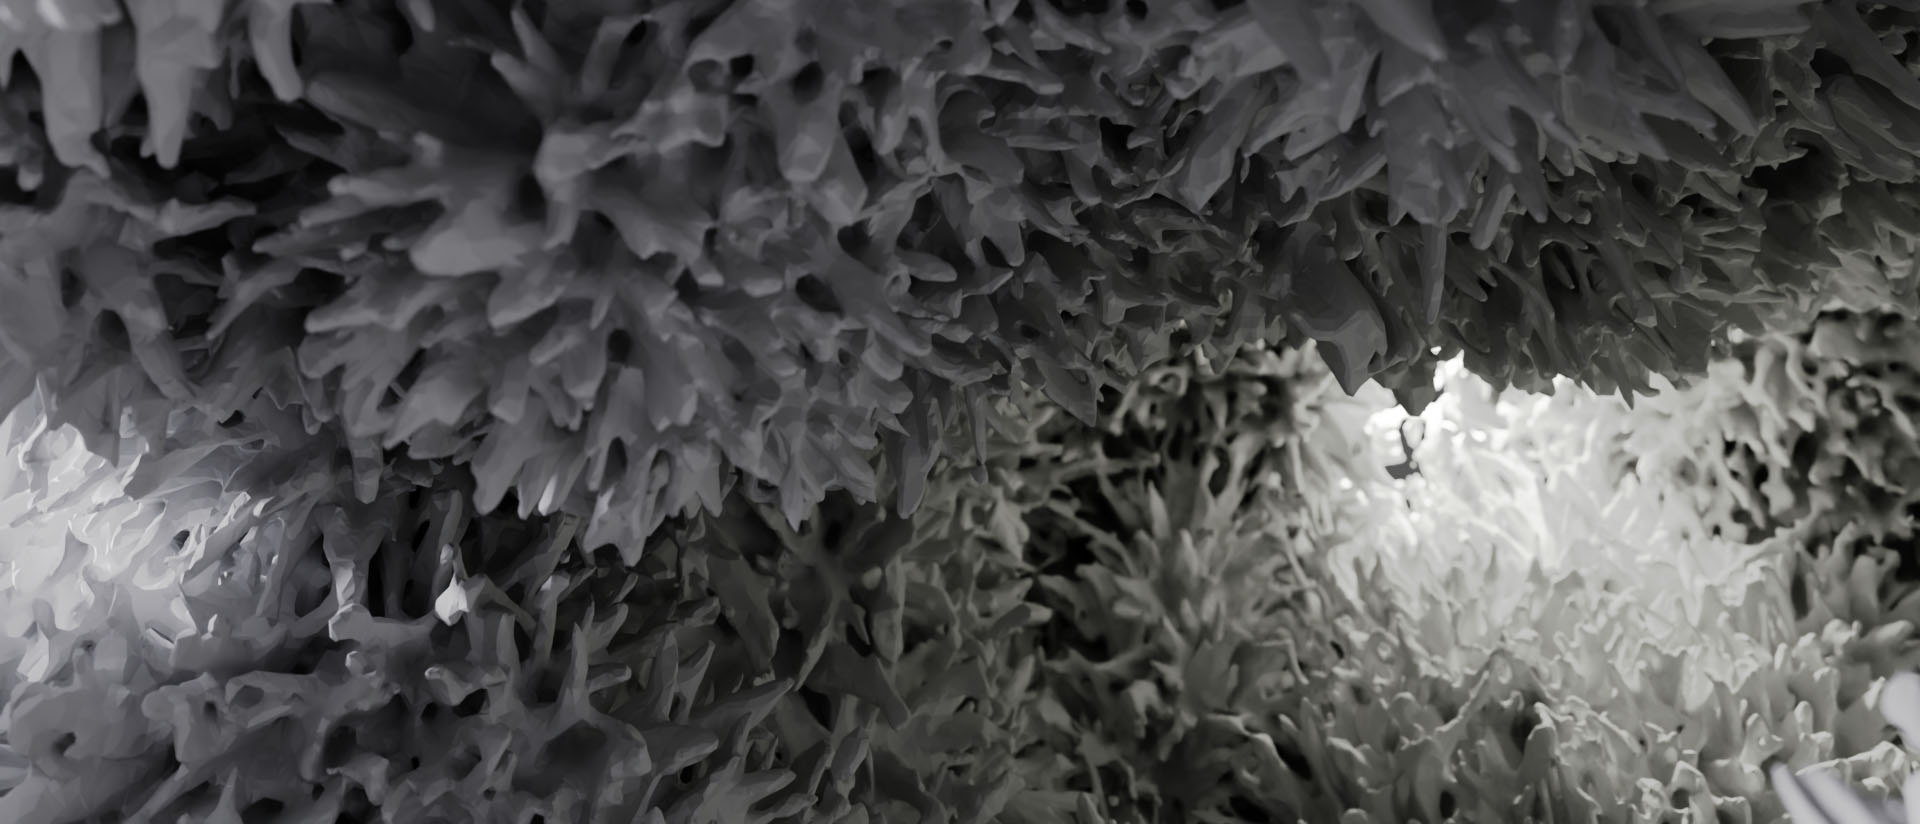
\includegraphics[width=\textwidth]{intro-anim/Animation06.jpg}
	\else
		\animategraphics[palindrome,autoplay,width=\textwidth]{6}{intro-anim/Animation}{01}{10}
	\fi
    \caption{Artistic 3D reconstruction of \acl*{CSH}-fibres within a capillary pore of \SI{28}{\day} hydrated \acl*{C3S}. The dataset was recorded using a \acl*{SEM} combined with a \acl*{FIB}. \cite{kleiner.2021c}}
    \label{fig:intro}
\end{figure*}

While the knowledge and measurement techniques have significantly improved within the last century, this is still true to a certain extent today.
Good knowledge of the structural development and therefore, reliable measurement and evaluation methods are crucial to understand, model \cite{nguyen-tuan.2023,nguyen-tuan.2024} and consequently influence the hydration of cements.
Good measurement and evaluation methods are therefore required.

A \ac{SEM} is a powerful tool to image the microstructure of a lot of materials.
Electron microscopy is widely known for its \ac{SE}-mode, which gives a great idea of the surface profile of the specimen, or the \ac{BSE}-mode resulting in a chemical contrast image.
Nevertheless, the data extracted from the resulting images can be greatly improved, if also data from \ac{EDX}, \ac{EBSD}, optical microscopy, \ac{mCT}, laser ablation or nano indentation are recorded.
The combination of multiple (imaging) techniques as the afore mentioned is often referred to as correlative microscopy.
It results in significantly more information than the simple sum of the individual method would be able to produce.

Therefore, this thesis is devoted to improve the characterization the micro-structure of unhydrated and hydrated cement based binders by combining a set of imaging techniques like \ac{SEM} and \ac{mCT} and comparing them to selected methods like \ac{LTDSC} and \ac{MIP}.
The goals are to better understand the influence of the devices and techniques, and finding improved ways to combine them to gain better knowledge about unhydrated and hydrated cements and the cement hydration, defining protocols and best practices to obtain statistical relevant data and to develop or adopt software tools for image analysis.
Furthermore, the composition of clinker and the structure and porosity of hydration products were the focus of this work.

Modern computer vision methods allow to develop complicated and creative evaluation methods, which were computational to expensive, just a few years ago.
Therefore, existing analytical methods are to be improved and further developed to be reproducible and and fairly easily repeatable.

Please note, that this work uses the cement chemist notation for most chemical equations (see Table~\ref{tab:ccn}).

% TODO: Christane:
% hier könnte schon noch so ein kleiner abriß stehen, dass man mit mikroskopie schon immer versucht materialien wie beton besser zu verstehen und eigenschaften verständlich bzw vorhersagbar zu machen. dass man dank moderner mikroskopie nun modelle entwickelnn kann um die mikrostrutur zu simulieren (sheet growth chapter hierher holen?, hymostruc oder eben auch 2D-3D transformation in zukunft dank ML blabla nutzen kann..)

{\color{red}
Chapter ideas
\begin{itemize}
	
	\item Dissolution- and hydration rates of clinker phases depending on the crystal orientation (SEM+EBSD+VSI)
	\item Chemical and structural 3D-analysis of hydrated cementitious materials
\end{itemize}
}

% Einleitung/Grundlagen:
% alles mit ausreichend Literatur belegen, sehr allgemein:
% Was ist Zement? Verwendung? Gesellschaftlicher Nutzen? Zeitlicher Kontext?

% spezieller Klinkerphasen/Bindemittel:
% Was sind Klinkerphasen? Wozu Binder? Alternativen?
% Wie werden beide methodisch untersucht?
% Unterschiede? Herausforderungen? Probenbehandlung?
% historische und moderne Methodik?
% 2D- und 3D-Methoden? Unterschiede? Vorteile?
		\chapter{Methods}

In this Dissertation, a myriad of different experimental and evaluation methods was used.
These methods will be detailed in this chapter.


\section{The preparation process for SEM}

To obtain high-quality images \ac{SEM} which allows for a systematical image analysis, very smooth surfaces are required.
Those surfaces can be achieved by mechanically polishing epoxy embedded specimens.


\subsection{mechanical polishing}

\begin{itemize}
\item
\end{itemize}


\subsection{Argon Broad Ion Beam Polishing (moving specimen)}

\blindtext

Description


\subsection{Argon Broad Ion Beam Polishing (fixed specimen)}

\blindtext


\section{SEM / Focussed Ion Beam}

\subsection{Energy-dispersive X-ray spectroscopy}

\subsection{Electron backscatter diffraction}

% depends on the future success with 3D FIB

\subsection{Serial sectioning using Focussed Ion Beam}


\section{Laser Ablation - Inductively Coupled Plasma - Mass Spectrometry}

\section{}
		\chapter{SEM and FIB-SEM analysis}

To obtain high-quality images scanning electron microscopy (SEM) which allows for a systematical image analysis, very smooth surfaces are required.
Those surfaces can be achieved by mechanically polishing epoxy embedded specimens.

\section{Damages induced by SEM}

show artifacts

\begin{itemize}
\item C-S-H beam damage (moving needles)
\item C-S-H beam damage (pore indroducing)
\end{itemize}


\section{Damages induced by FIB-SEM}
		\chapter{CT}

(maybe not?)


		\printbibliography[title={Bibliography}]  % print bibliography


	\appendix  % begin appendix
		\chapter{Appendix}

\ifdefined\DRAFT
{
\color{red}
Figures in the appendix section are not visible in draft mode!
}
\fi

\section{Hydrate rim measurements}

\begin{figure*}[htb!]
    \centerline{\includegraphics[width=\textwidth]{hydrate-rim/supplementary/threshold_types.pdf}}
    \caption{Segmentation results of 14 days hydrated alite. Raw image (A); segmentation result by thresholding (B), pixel classification (C) and manual segmentation (D). Grey: raw data; blue: alite; green: hydrates (C and D only dense C-S-H); red: CH; yellow: outer C-S-H.\label{fig:results_segmentation_methods}}
\end{figure*}

\begin{figure}[htbp]
	\centerline{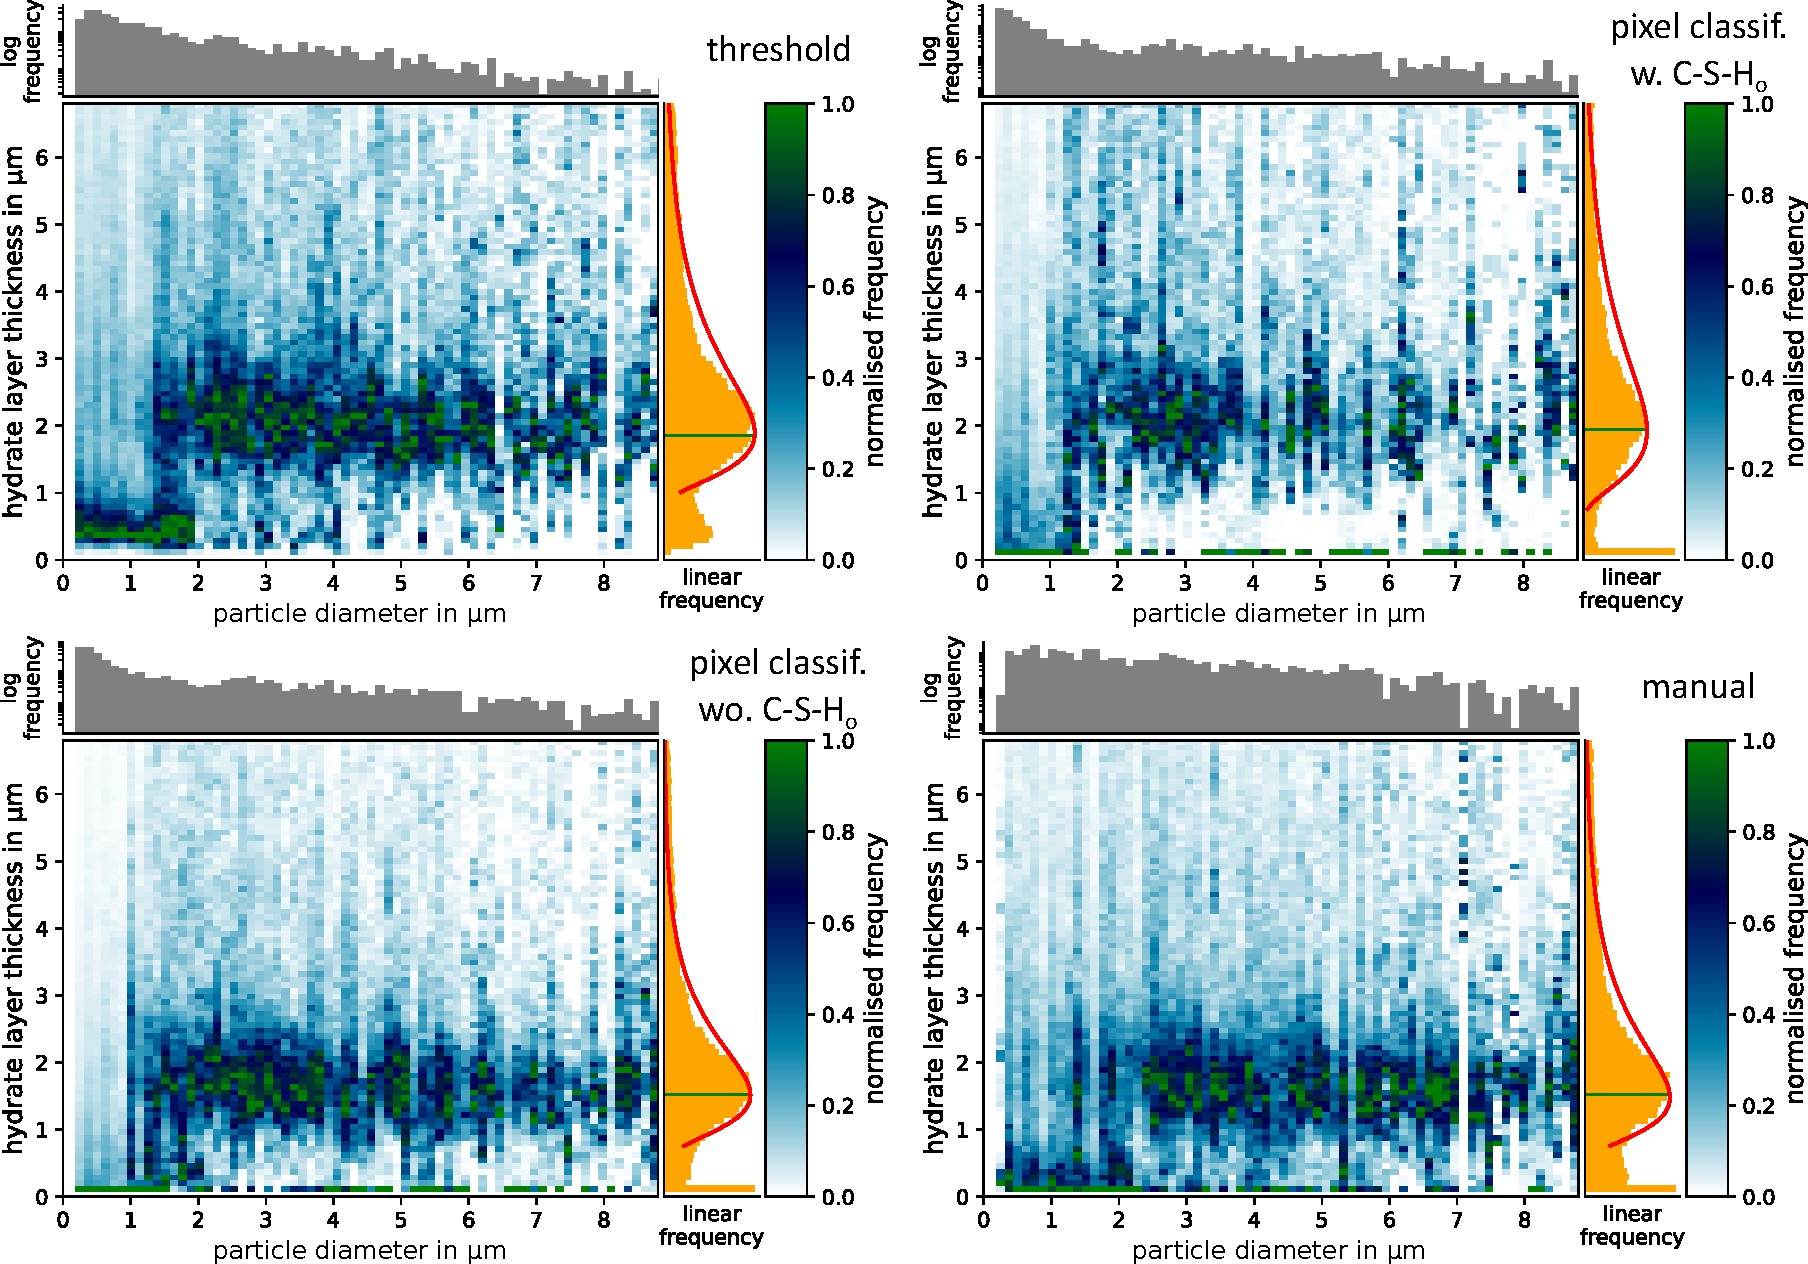
\includegraphics[width=\textwidth]{hydrate-rim/histogram_segmentation2.pdf}}
	\caption{Histograms of the hydration layers of \SI{14}{\day} hydrated alite. Segmentation result by thresholding ($l_\text{max}$ = \SI{1.85}{\micro\meter}), pixel classification with ($l_\text{max}$ = \SI{1.94}{\micro\meter}) and without respecting \ac{CSHo} ($l_\text{max}$ = \SI{1.52}{\micro\meter}) and manual segmentation ($l_\text{max}$ = \SI{1.52}{\micro\meter})
	Same diagram type as in Figure~\ref{fig:results2d_alite}. \label{fig:hlt_segmentation_influence}}
\end{figure}

\begin{figure}[htbp]
	\centerline{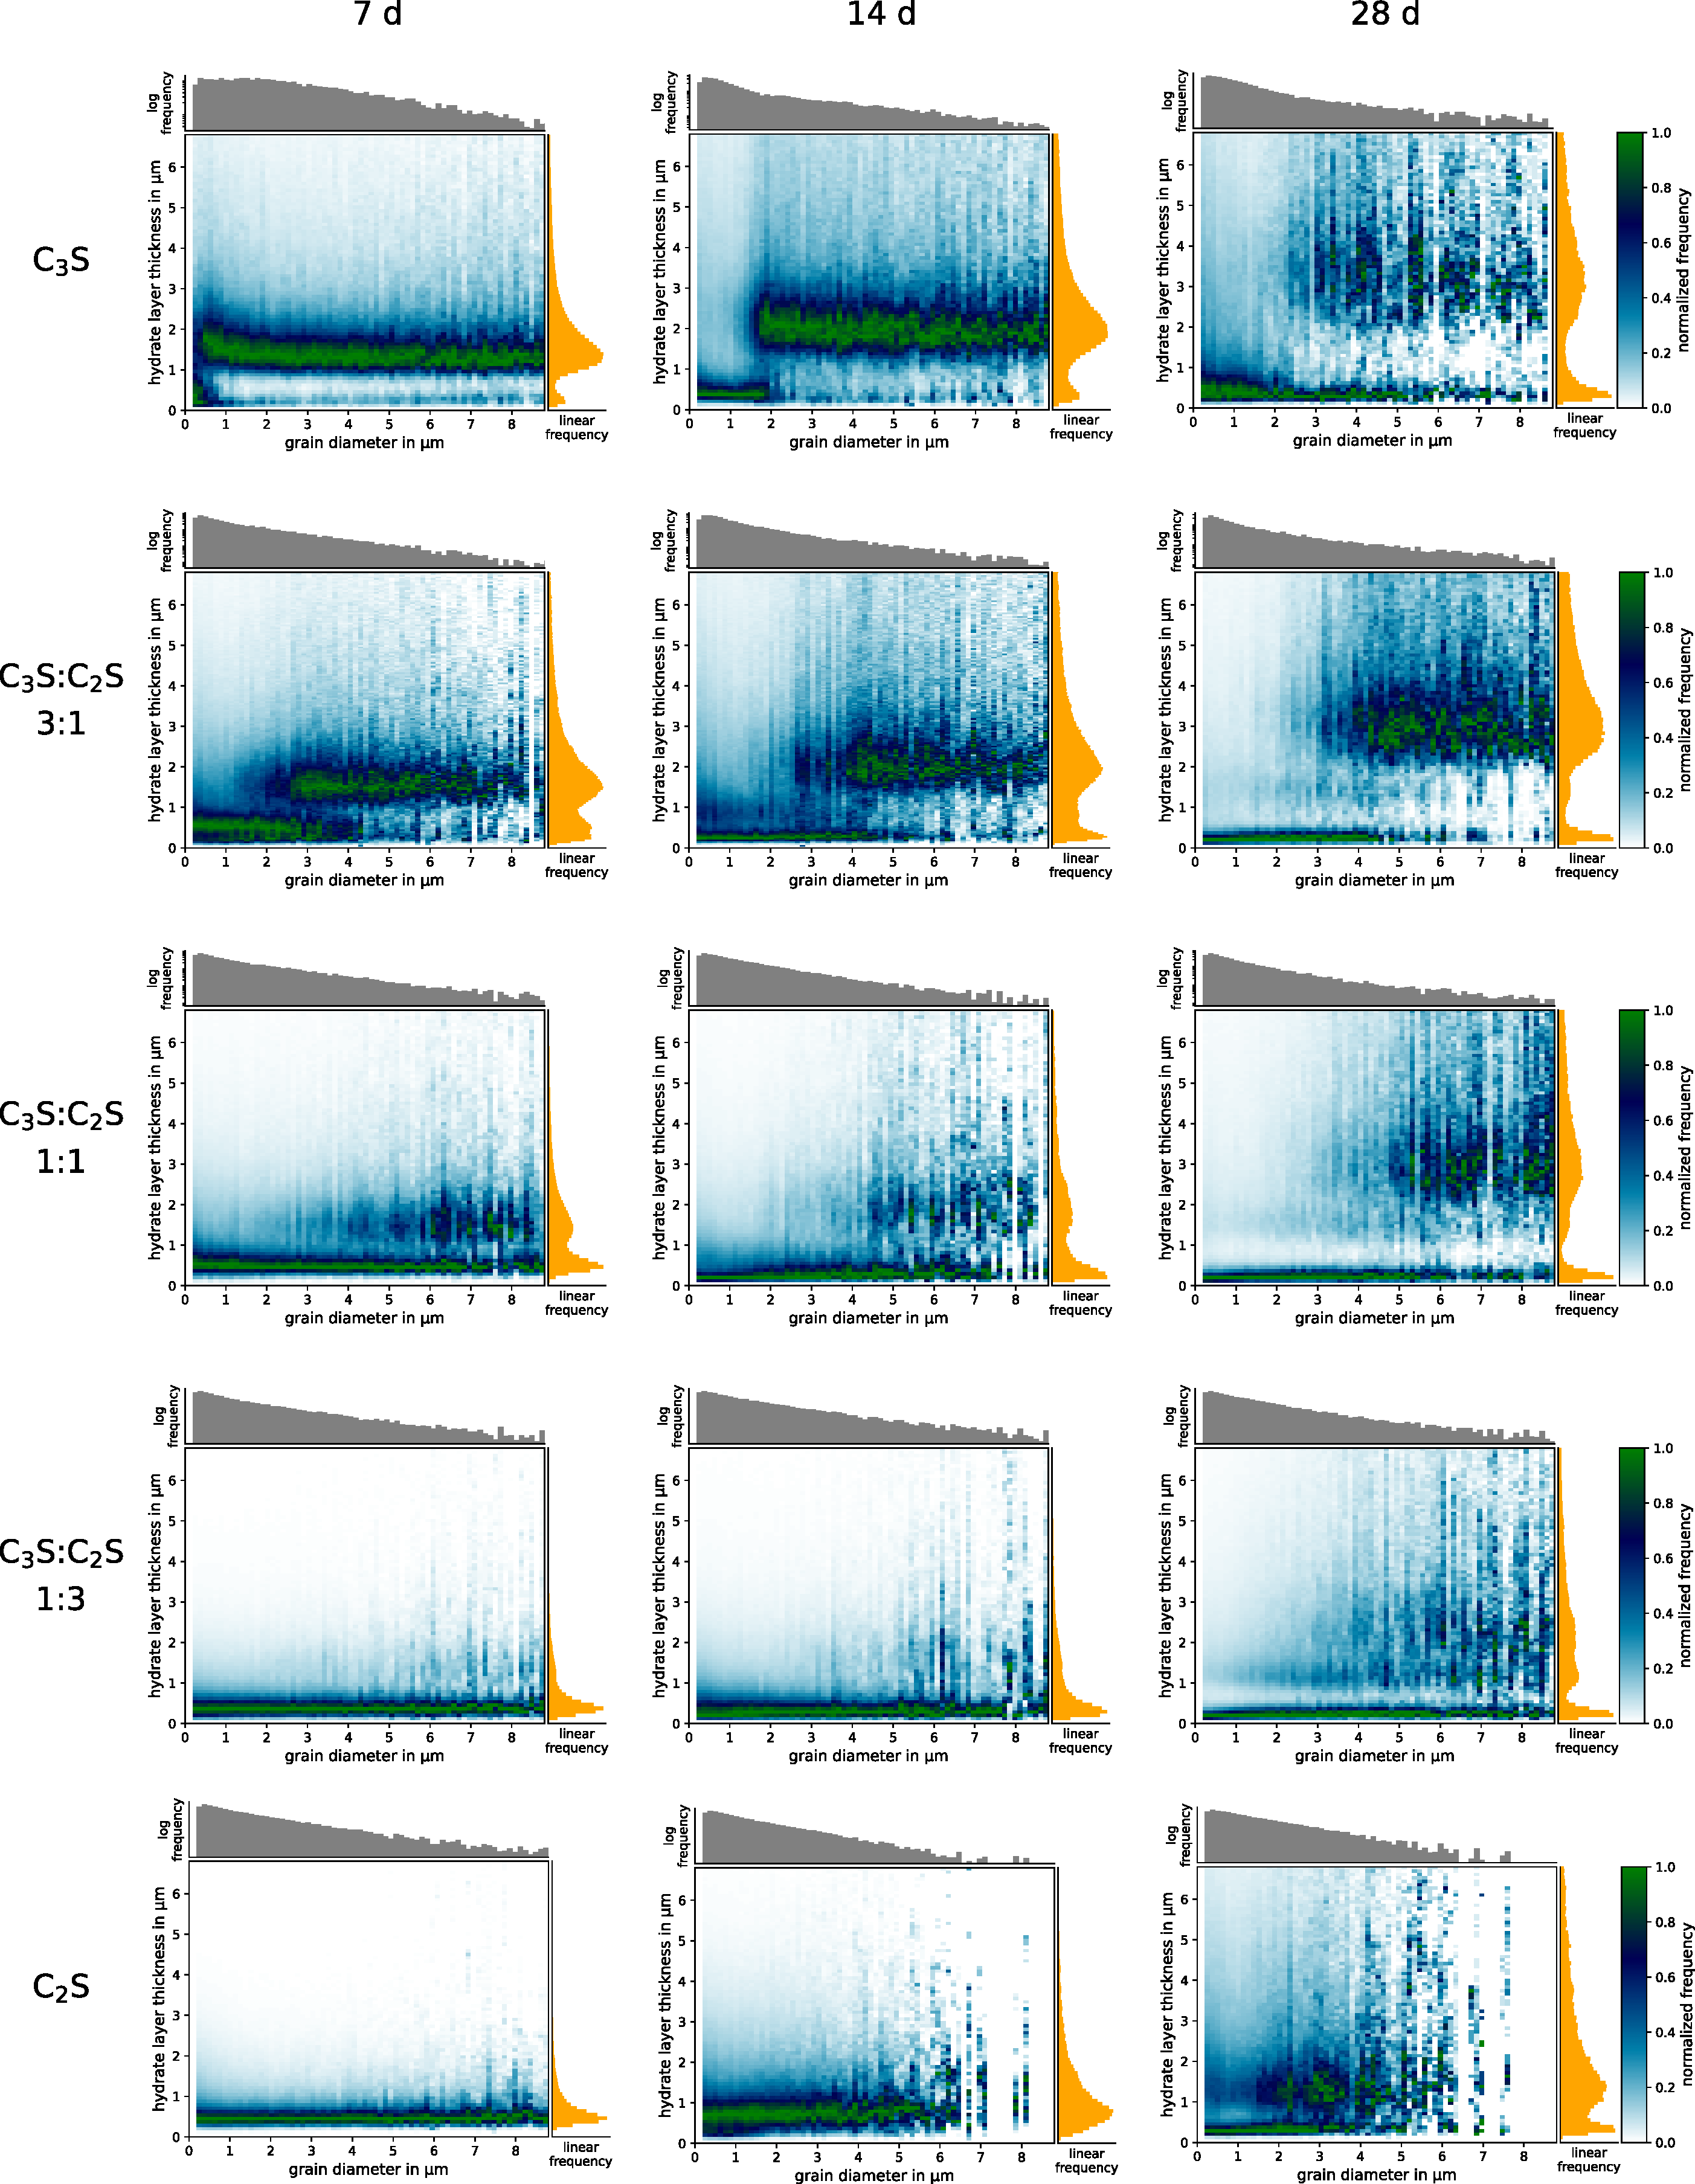
\includegraphics[width=\textwidth]{hydrate-rim/supplementary/mixture_overview.pdf}}
	\caption{Normalized distributions of the \ac{HLT} of hydrated alite, belite and mixtures (aged 7, 14, and \SI{28}{\day}) depending on the particle diameter.
	Same diagram type as in Figure~\ref{fig:results2d_alite}.
	\label{fig:results2d_belite}}
\end{figure}  % include appendix content

	\chapter{Ehrenwörtliche Erklärung}

Ich erkläre hiermit ehrenwörtlich, dass ich die vorliegende Arbeit ohne unzulässige Hilfe Dritter und ohne Benutzung anderer als der angegebenen Hilfsmittel angefertigt habe.
Die aus anderen Quellen direkt oder indirekt übernommenen Daten und Konzepte sind unter Angabe der Quelle gekennzeichnet.

Bei der Auswahl und Auswertung folgenden Materials haben mir die nachstehend aufgeführten Personen in der jeweils beschriebenen Weise unentgeltlich geholfen:

\ifdefined\PRINTABLE
  \begin{itemize}
    \item \textit{Fachliche Betreuung und Korrektur:} Dr. rer. nat. Christiane Rößler und Prof. Dr.-Ing. Horst-Michael Ludwig
    \item \textit{Einzelne REM-Analysen:} Dipl.-Ing. Christian Matthes und Dr. rer. nat. Christiane Rößler
    \item \textit{Probenpräparation:} Dipl.-Chem. Nadine Brendel und Lydia Schmiedel
    \item \textit{\acs*{LAICPMS}-Messungen:} Dr.-Ing. Marco Decker und Prof. Harald Hilbig
    \item \textit{\acs*{XRD}-Messungen:} M. Sc. Franz Becker und Prof. Dr. Jürgen Neubauer
    \item \textit{Nanoindentationsversuche:} M. Sc. Feng Li
    \item \textit{\acs*{fs-laser}-Präparation:} Prof. Dr. Thomas Höche und M. Sc. Georg Schusser
    \item \textit{Korrekturlesen:} Dr. rer. nat. Michael Böhme, M. Sc. Sophie Unbehau und Dr. rer. nat. Thomas Sowoidnich
  \end{itemize}
\else
  \begin{itemize}
    \item \textit{Fachliche Betreuung und Korrektur:} \withORCID[0000-0002-8420-4849]{Dr. rer. nat. Christiane Rößler} und \withORCID[0000-0002-8998-4936]{Prof. Dr.-Ing. Horst-Michael Ludwig}
    \item \textit{Einzelne REM-Analysen:} Dipl.-Ing. Christian Matthes und \withORCID[0000-0002-8420-4849]{Dr. rer. nat. Christiane Rößler}
    \item \textit{Probenpräparation:} Dipl.-Chem. Nadine Brendel und Lydia Schmiedel
    \item \textit{\acs*{LAICPMS}-Messungen:} Dr.-Ing. Marco Decker und \withORCID[0000-0002-2002-2026]{Prof. Harald Hilbig}
    \item \textit{\acs*{XRD}-Messungen:} \withORCID[0000-0003-1993-1983]{M. Sc. Franz Becker} und Prof. Dr. Jürgen Neubauer
    \item \textit{Nanoindentationsversuche:} \withORCID[0009-0007-9412-7529]{M. Sc. Feng Li}
    \item \textit{\acs*{fs-laser}-Präparation:} \withORCID[0000-0003-0117-8495]{Prof. Dr. Thomas Höche} und M. Sc. Georg Schusser
    \item \textit{Korrekturlesen:} \withORCID[0000-0003-2097-4657]{Dr. rer. nat. Michael Böhme}, \withORCID[0009-0008-2837-7623]{M. Sc. Sophie Unbehau} und \withORCID[0000-0002-9761-672X]{Dr. rer. nat. Thomas Sowoidnich}
  \end{itemize}
\fi


Zur sprachlichen Korrektur (Rechtschreibung, Grammatik) der Texte wurde generative KI (\textsc{Google Gemini}, \textsc{DeepL}) verwendet.
Alle so angepassten Textkorrekturen wurden vor der Einarbeitung in die Arbeit manuell geprüft.
Für die Erstellung, Korrektur (\acs*{EBSD}-Auswertung) und Optimierung (Hydratsaummessung) einiger Python-Skripte  wurde generative KI eingesetzt (\textsc{Google Gemini}, \textsc{Cursor}).
Der Code wurde vollständig von mir gereviewt und validiert.

Weitere Personen waren an der inhaltlich-materiellen Erstellung der vorliegenden Arbeit nicht beteiligt. 
Insbesondere habe ich hierfür nicht die entgeltliche Hilfe von Vermittlungs- bzw. Beratungsdiensten (Promotionsberater oder anderer Personen) in Anspruch genommen.
Niemand hat von mir unmittelbar oder mittelbar geldwerte Leistungen für Arbeiten erhalten, die im Zusammenhang mit dem Inhalt der vorgelegten Dissertation stehen.

Die Arbeit wurde bisher weder im In- noch im Ausland in gleicher oder ähnlicher Form einer anderen Prüfungsbehörde vorgelegt.

Ich versichere ehrenwörtlich, dass ich nach bestem Wissen die reine Wahrheit gesagt und nichts verschwiegen habe.

  \vspace{1cm}

  Weimar, den \todayde \par

  \vspace{2cm}

  Florian Kleiner


\end{document}
